% Created 2020-09-28 lun 19:05
% Intended LaTeX compiler: pdflatex
\documentclass[presentation,aspectratio=169, usenames, dvipsnames]{beamer}
\usepackage[utf8]{inputenc}
\usepackage[T1]{fontenc}
\usepackage{graphicx}
\usepackage{grffile}
\usepackage{longtable}
\usepackage{wrapfig}
\usepackage{rotating}
\usepackage[normalem]{ulem}
\usepackage{amsmath}
\usepackage{textcomp}
\usepackage{amssymb}
\usepackage{capt-of}
\usepackage{hyperref}
\usepackage{khpreamble}
\usepackage{amssymb}
\usepgfplotslibrary{groupplots}
\usepackage{pgfplotstable}
\newcommand*{\shift}{\operatorname{q}}
\definecolor{ppc}{rgb}{0.1,0.1,0.6}
\definecolor{iic}{rgb}{0.6,0.1,0.1}
\definecolor{ddc}{rgb}{0.1,0.6,0.1}
\usetheme{default}
\author{Kjartan Halvorsen}
\date{2020-09-28}
\title{Control Engineering Laboratory - Cascade control and feed forward}
\hypersetup{
 pdfauthor={Kjartan Halvorsen},
 pdftitle={Control Engineering Laboratory - Cascade control and feed forward},
 pdfkeywords={},
 pdfsubject={},
 pdfcreator={Emacs 26.3 (Org mode 9.3.6)}, 
 pdflang={English}}
\begin{document}

\maketitle

\section{Context and main idea}
\label{sec:orgf16c449}
\begin{frame}[label={sec:org8d5908e}]{The two-tank model with one level sensor}
\begin{center}
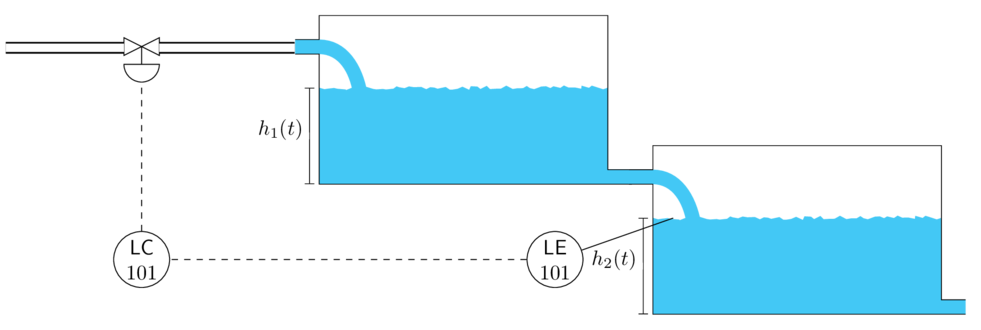
\includegraphics[width=\linewidth]{../../figures/two-tanks-shutoff-valve}
\end{center}
\end{frame}

\begin{frame}[label={sec:orge7e62fe}]{The two-tank model with two level sensors and one flow sensor}
\begin{center}
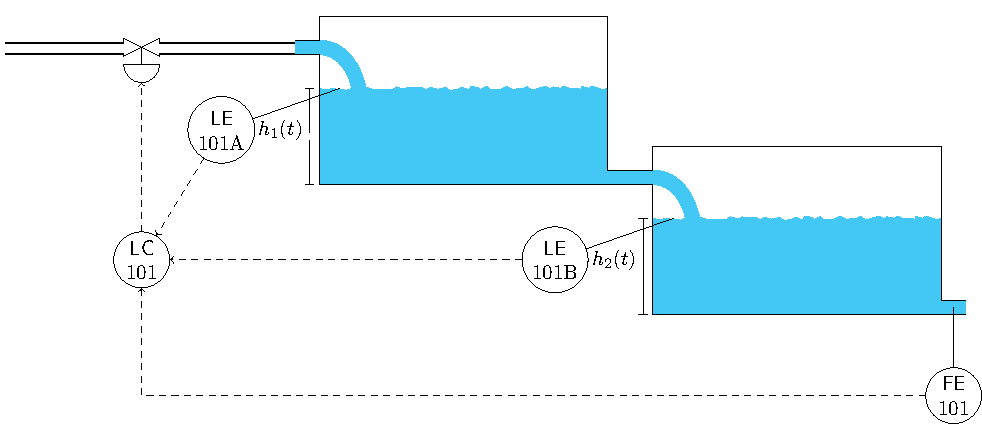
\includegraphics[width=\linewidth]{../../figures/two-tanks-2LE-FE}
\end{center}

\alert{Key idea: We can improve the control using more information}
\end{frame}

\section{Cascade control}
\label{sec:org4a6df0b}
\begin{frame}[label={sec:org4fa23f0}]{Cascade control}
\begin{center}
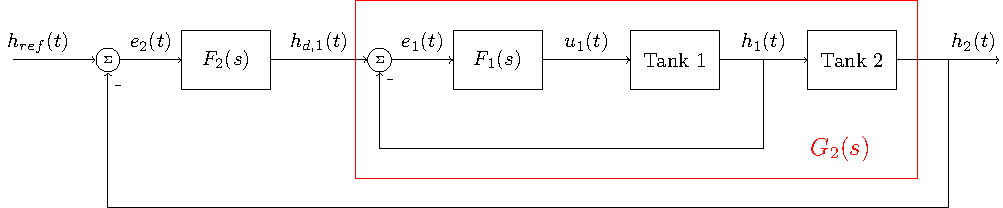
\includegraphics[width=\linewidth]{../../figures/block-diagram-cascade-control.pdf}
\end{center}
\end{frame}

\begin{frame}[label={sec:orga6e9544}]{Designing the inner loop}
\begin{center}
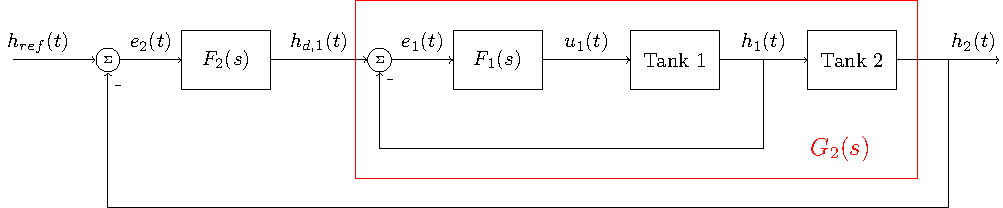
\includegraphics[width=0.6\linewidth]{../../figures/block-diagram-cascade-control.pdf}
\end{center}
Have model \(G_1(s) = \frac{K_1}{s\tau_1 + 1} = \frac{51}{51s + 1}\). PI controller \[F_1(s) = k_{c} \left( 1 + \frac{1}{\tau_{i}s}\right) = k_{c} \frac{\tau_{i}s + 1}{\tau_{i}s}\]
Characteristic equation
\[ s(s\tau_1 + 1) + k_c \frac{K}{\tau_{i}}(s\tau_{i} + 1) = 0\]
Choose \(\tau_i\) and \(k_c\) to place the poles at any desired location in the LHP. 
\end{frame}

\begin{frame}[label={sec:org4059860}]{Exercise}
Have characteristic equation
\[ s(s\tau_1 + 1) + k_c \frac{K}{\tau_{i}}(s\tau_{i} + 1) = 0\]

\alert{Choose \(\tau_i = \tau_1\), and then determine \(k_c\) which gives a pole in \(s=-\frac{4}{\tau_1}\).}
\end{frame}

\begin{frame}[label={sec:org12b38e8}]{Designing the outer loop}
\begin{center}
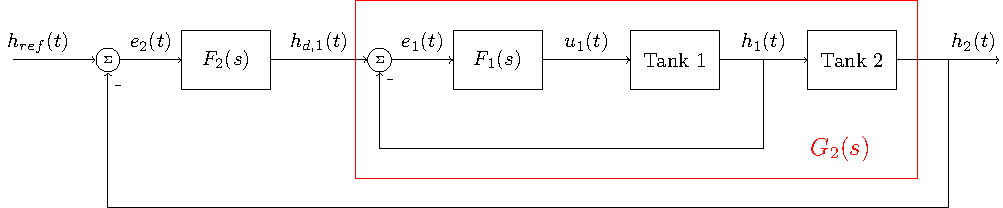
\includegraphics[width=0.6\linewidth]{../../figures/block-diagram-cascade-control.pdf}
\end{center}
The output of the outer controller \(F_2(s)\) is the desired level in tank 1. If the inner loop is sufficiently fast, we can approximate that the actual level in tank 1 is equal to the desired level. 

\begin{center}
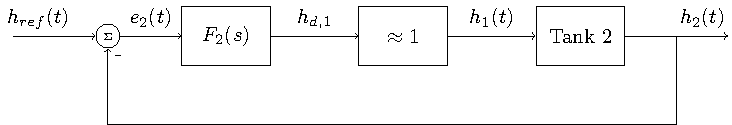
\includegraphics[width=0.9\linewidth]{../../figures/block-diagram-cascade-outer-loop}
\end{center}
\end{frame}



\begin{frame}[label={sec:orgc28b7f7}]{Designing the outer loop, contd}
Alternatively, we can fit a model to the plant and the inner control-loop
\begin{center}
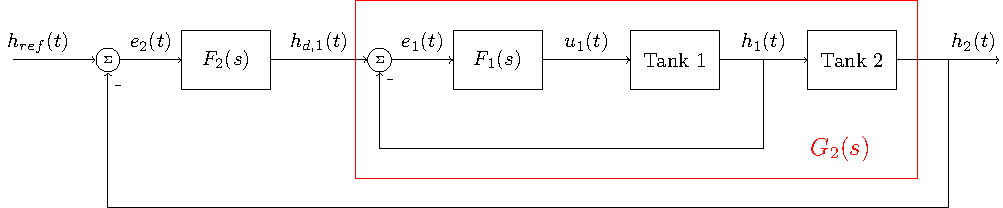
\includegraphics[width=0.9\linewidth]{../../figures/block-diagram-cascade-control-G2}
\end{center}
\end{frame}


\section{Feed forward from the disturbance}
\label{sec:org620b1fc}

\begin{frame}[label={sec:orga9aa4df}]{Feed forward from the disturbance}
\begin{center}
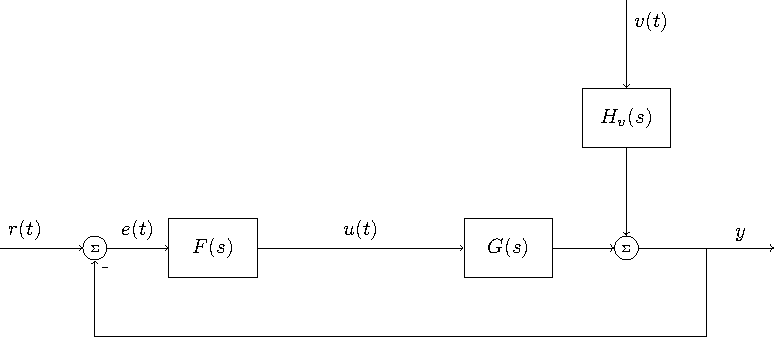
\includegraphics[width=\linewidth]{../../figures/block-diagram-ffw-no-ffw}
\end{center}
\end{frame}

\begin{frame}[label={sec:org3e09e8f}]{Feed forward from the disturbance}
\begin{center}
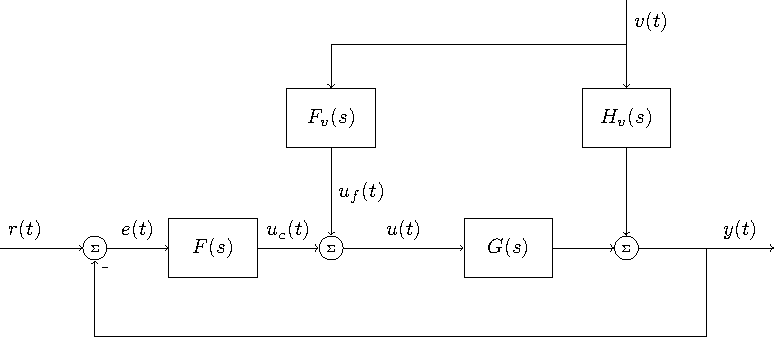
\includegraphics[width=\linewidth]{../../figures/block-diagram-ffw}
\end{center}
\end{frame}

\begin{frame}[label={sec:org2551c79}]{Feed forward from the disturbance}
\begin{center}
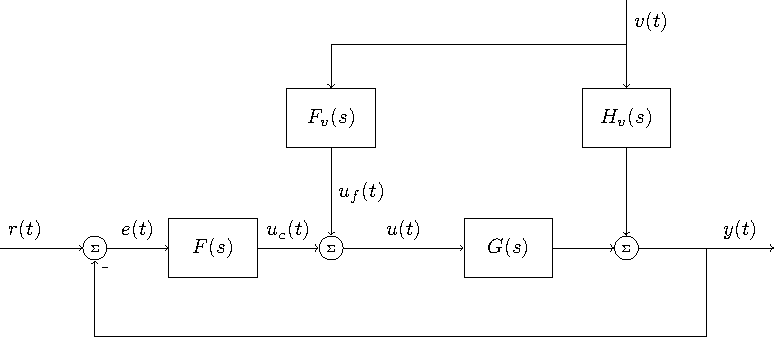
\includegraphics[width=0.7\linewidth]{../../figures/block-diagram-ffw}
\end{center}

Clearly,
\[ Y(s) = H_V(s)V(s) + G(s)\Big(U_C(s) + F_v(s)V(s)\Big)\]
\alert{Activity: Determine \(F_v(s)\) that eliminates the effect of the disturbance!}
\end{frame}
\end{document}